\documentclass[a4paper]{article}

\usepackage[
            pdfpagelabels=true,
            a4paper,
            bookmarks=true,
            bookmarksnumbered=true,
            bookmarksopen=true,
            bookmarksopenlevel=1,
            breaklinks=true,
            colorlinks=true,
            hyperindex=true,
            linkcolor=black, %blue, %default: red
            citecolor=black,
            urlcolor=blue,
            pdfpagelayout=SinglePage,
            ]{hyperref}

\usepackage[utf8]{inputenc}
\usepackage[T1]{fontenc}

\usepackage{graphicx}
\graphicspath{{graphics/}}
\usepackage{subfig}
\usepackage{mathtools}
\usepackage{url}

\usepackage{todonotes}




\hypersetup{
            pdftitle={Neverblender Documentation},
            pdfauthor={-},
            pdfkeywords={Blender, Neverwinter Nights, NWN, neverblender},
            pdfsubject={}
}

\begin{document}

\title{Neverblender Manual}

\date{\today}

\maketitle
\tableofcontents

\section{Installation}

\subsection{Requirements}
The only requirement is Blender 2.6x. It will not work with 2.5x or earlier versions.

\subsection{Installation}
Put the Neverblender folder into the scripts/addons directory of your Blender directory. Open blender and navigate to File, User Preferences, Addons and enable Neverblender by ticking the check box (It is located under Import-Export category). Make sure to click on the {\itshape{Save as Default}} Button, if you want Neverblender to be enabled by default, else you will have to re-enable it after every startup.


\section{Import \& Export}

\subsection{Import}

\subsubsection*{Import Options}

\begin{figure}
  \centering
  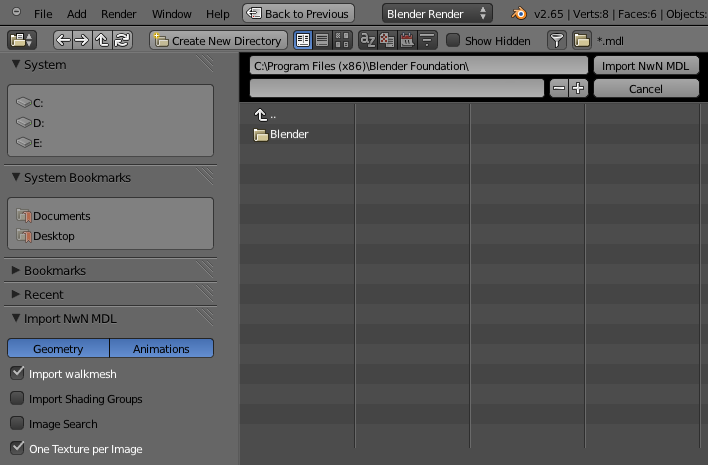
\includegraphics[trim=0 0 0 0, clip, width=\textwidth]{import01}
  \caption[mdl import]{Import Screen}
  \label{fig:import01}
\end{figure}

\begin{description}
    \item[Geometry \& Animation] Either import the geometry, animations or both. Note that the animations may not work, if the animated objects are not present. However you may add the animations to other objects manually.
    \item[Import Walkmesh] Attempts to import a walkmesh. If the imported model is a placeable, the script will look for a {\itshape{*.pwk}} file in the same folder. If the model is a door, it will look for a {\itshape{*.dwk}} file. If the model is a tile, it will read the walkmesh directly from the {\itshape{*.mdl}} file.
    \item[Import Shading Groups] Import shading groups for faces. Shading groups are not supported by Blender, i.e. it will have no effect on the displayed model in blender. An imported shading group is converted to a vertex group, containing all vertices of the faces belonging the shading group.
    \item[Image Search] Enable this to search for textures in subdirectories. (This may be slow)
    \item[One Texture per Image] When this is enabled, the import script will create only one texture for every image found in the model file. When disabled, every node will get it's own texture, even if it's image has already been loaded to a different texture previously.
\end{description}

\subsubsection*{Animation Import}
For each animation in the imported model, the export script will create a new scene and copy the required objects from the original scene into the new scene. The objects are full copies, but editing the mesh in one of the animation scenes will have no effect on the exported model.

If no geometry was imported and the animated objects are not already present, the animations will be imported as actions only. The actions will be named {\itshape{animation\_name.object\_name}} and you may assign them to objects yourself at a later time in the action editor.

Please note that blender does not display some animations correctly if they are imported (namely: color keys), but will nevertheless export them.

\subsection{Export}

\subsubsection*{Export Options}
\begin{description}
    \item[Export] This only refers to the aurora base object (MDLBASE). All children of the base object will be exported regardless of this setting.
    \item[Export Walkmesh] Attempts to export a walkmesh. If the imported model is a placeable or door the script will look for a PWKBASE or DWKBASE object in the current scene. If the model is a tile it will look for aabb walkmesh object parented to the MDLBASE. If no walkmesh is found, the model itself will still be exported as {\itshape{*.mdl }} file.
    \item[Apply Modifiers] Apply Modifiers before exporting. (For example: If a mirror modifier is used, this option should be checked or else the objects may not be exported as displayed in the 
3D View)
    \item[Export Shading Groups] Export Shading Groups. Shading groups will be generated from the corresponding vertex groups. If a face has been assigned to more than one shading group, a random  shading group will be chosen. 
\end{description}

\section{Editing}
This Section covers all additional properties, added by Neverblender. The aurora property panel can be accessed by opening the property panel of an object and selecting the object data panel, as show in figure~\ref{fig:meshprops01}

\begin{figure}
  \centering
  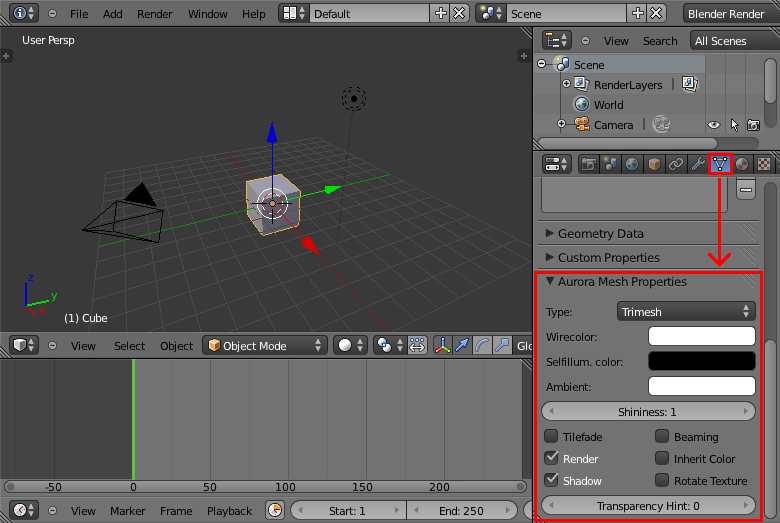
\includegraphics[trim=0 0 0 0, clip, width=\textwidth]{meshprops01}
  \caption[mdl import]{Accessing the aurora property panel added by Neverblender}
  \label{fig:meshprops01}
\end{figure}

\subsection{Dummy Nodes}
Dummy nodes are represented as {\itshape{Empties}}. {\itshape{Empties}} are Null objects and contain no geometry. (see  \hyperref{http://wiki.blender.org/index.php/Doc:2.6/Manual/Modeling/Empties}{}{}{Empties in the blender manual}).

There are three specific types of dummies selectable in the aurora property panel:
\begin{description}
    \item[mdl base] The model base, aurora base or rootdummy. All objects should be directly or indirectly parented to this {\itshape{Empty}} with the only exception being the door walkmesh and the placeable walkmesh. Only the objects parented to this {\itshape{Empty}} will be saved in the {\itshape{*.mdl}} file upon export.
    \item[dwk base] The door walkmesh must be parented to an {\itshape{Empty}} with this type. They only serve as walkmesh  and will be saved as {\itshape{*.dwk}} file upon export. A dwk base dummy has no additional properties.
    \item[pwk base] The placeable walkmesh must be parented to an {\itshape{Empty}} with this type. Objects parented to this object are never displayed, they only serve as walkmesh and will be saved as {\itshape{*.pwk}} file upon export. A pwk base dummy has no additional properties.
\end{description}
Each of these can only be used once for a single model. However it is possible to add other dummies to the model without a specific type.

\subsubsection{Aurora Base or Rootdummy}

\subsection{Meshes}


\subsubsection{Trimeshes}
A newly created mesh object is a trimesh by default, the most common type of mesh used by the aurora engine. While the aurora engine only accepts triangles as faces, you may use ngons during editing in blender. During export, all faces will be converted to triangles and the uv coordinates adjusted accordingly.

\begin{description}
    \item[Wirecolor] 
    \item[Self-illumination color]
    \item[Ambient Color] 
    \item[Shininess]
    \item[Tilefade]
    \item[Render]  
    \item[Shadow]
    \item[Beaming]
    \item[Inherit Color]  
    \item[Rotate Texture]
    \item[Transparency hint]      
\end{description}

%trim=l b r t
\begin{figure}%
  \centering
\subfloat[Danglymesh]{\label{fig:danglymesh01}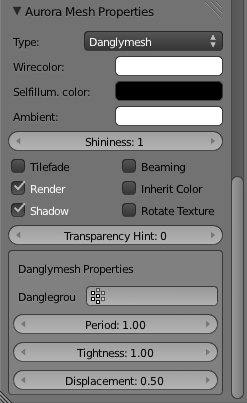
\includegraphics[width=0.40\textwidth]{danglymesh01}}\qquad
\subfloat[Skinmesh]{\label{fig:skinmesh01}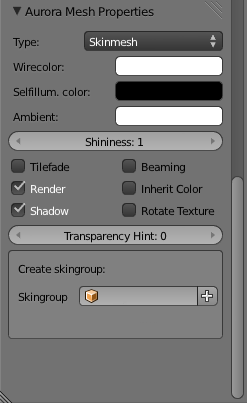
\includegraphics[width=0.40\textwidth]{skinmesh01}}
\caption[Additional Porperties]{Additional properties for danglymeshes and skinmeshes}%
  \label{fig:addprops}%
\end{figure}

\subsubsection{Danglymeshes}
In addition to the trimesh properties Danglymeshes have some additional properties:
\begin{description}
    \item[Dangle group] The dangle group is a vertex group containing the weights of vertices for the danglymesh. You must select an existing vertex group.
    \item[Period] 
    \item[Tightness]
    \item[Displacement] 
\end{description}

\subsubsection{Skinmeshes}
In addition to the trimesh properties, skin meshes also offer the option to add skin groups to the selected object. Skin groups are nothing more than vertex groups. The export script will recognize a vertex group as a skin group, if the group has the same name as an object in the scene.

There a two ways to add skin groups:
\begin{enumerate}
  \item Using the object selector found under the object properties you can select an object. A vertex group with the corresponding name will then be added automatically.
  \item Add a new vertex group with a name matching an object in the scene. The export script will then recognize it as a skin group.
\end{enumerate}

\subsubsection{aabb Walkmesh}
The walkmesh must be parented to the the {\itshape{mdl base}} object. No overlapping faces are allowed. To specify the surface type, it is necessary to add the walkmesh materials to the object. You can add all walkmesh materials by clicking on the {\itshape{Load walkmesh materials}} Button in the Aurora mesh properties panel. The walkmesh materials are then added as materials slots and accessible through the materials tab in the object properties. \\ \\
The export script will create an aabb tree from the walkmesh during export and save it the {\itshape{*.mdl}} file. It will also create a matching {\itshape{*.wok}} file.



\subsection{Lights}

\subsection{Animations}

\subsection{Emitter}
Unfortunately Neverblender offers very limited support for emitters, due to the fact that blenders particle system is too different from the system used in 3ds max.
\section{Tutorials}

\subsection{Blender}
\begin{description}
    \item[cgcookie.com] offers an introduction to blender (\url{http://cgcookie.com/blender/get-started-with-blender/}) as well as some more advanced tutorials.
    \item[blendtuts.com] offers Introduction to the blender 2.5 user interface \url{http://www.blendtuts.com/2010/06/blender-25-interface.html}. You should also check out the other tutorials.
    \item[Blender 3D Design Course] on \url{http://gryllus.net/Blender/3D.html} has a complete introduction to modeling with Blender aimed at beginners.
\end{description}

\subsection{Neverblender}
No Tutorials for Neverblender are available so far.

\section{Minimap Creation Tool}
The minimap creation tool can be downloaded separately and will automatically create minimaps for a tileset. The model files and textures of the tileset must be placed in the {\itshape{in}}  folder. Make sure the textures are in {\itshape{*.tga}} format. The {\itshape{*.set}} file is not necessary. \\ \\
The resulting minimaps will be in {\itshape{*.tga}} file format, without run Run-length encoding (RLE) and without alpha channel (RGB only). Transparency within the model will be displayed correctly. By default, no light sources from within the model are imported. Instead they are replaced with a single light source sitting above the center of the tile. Orthogonal projection is used for rendering.

\subsection{Prerequisites}
For the minimap creation tool to work correctly you will need blender 2.6x with an enabled Neverblender add-on. Make sure to enabled it by default, as the minimap tool uses operators from the add-on.

The path to the blender executable has to be specified in the {\itshape{generator.ini}} before usage.

\subsection{Options}
You can specify some of the render options in the {\itshape{generator.ini}} :
\begin{description}
\item[MINIMAP SIZE] Specifies the size of the rendered minimap in pixels. Minimaps are always square.
\item[Z OFFSET] This affects the z position of the camera used for rendering. You may need to set an z offset, in case your tileset contains very high objects or is far above zero level. The default camera height is 20.0 units.
\item[LIGHT COLOR] A single light source will be placed above the center of the tile. 
You can change the color of this light. The color has to be given in RGB format (values ranging from 0.0 to 1.0), separated by colons (without whitespaces)
\item[IMPORT LIGHTS] Whether to import the light sources from the models. It is not recommended
to do so. The color of the light sources may affect the render result, while in the engine their color is ignored and instead depending on the settings made by the builder.
\end{description}







\end{document}